\documentclass[a4paper, 11pt]{article}
\usepackage[utf8]{inputenc}
%\usepackage[margin=1in]{geometry}
\usepackage{graphicx}
\usepackage{listings}
\usepackage[hidelinks]{hyperref}
\usepackage{url}

\begin{document}

\begin{titlepage}
\begin{center}
\vspace*{1cm}

\huge{\textbf{Resource provisioning of containers}}

\Large{CS695 Project}

\vspace{3.5cm}
\Large{Department of Computer Science and Engineering}

\Large{IIT Bombay}

\vspace{1.5cm}

\Large{Anshul Gupta (16305R001) \\ Khursheed Ali (163059009)}

\vspace{1cm}
\today
\vfill

\vspace{0.8cm}


\includegraphics[scale=0.6]{IITB.png}
\end{center}
\end{titlepage}

\newpage
\tableofcontents
\newpage

\section{Problem Context}
\indent \indent Virtualization provides significant benefits over conventional implementation of operating systems by enabling dynamic virtual machine resizing and migration to eliminating hotspots.

The problem of resource provisioning in a cluster of VMs have already been addressed in a lot of papers and tools for example SandPiper \cite{sandpiper} or Memory Management in ESX Server \cite{memmgmt}. Since containers are relatively new, not much work have been done on their resource provisioning.

Containers present a different approach of isolation and virtualization. Containers being light-weight can easily be used for Platform-as-a-Service. With the ease of management, cluster administrator can effectively perform resizing and migration on containers. But manual hotspot detection can not only be cumbersome, it can also be ineffective as manual detection and resolution takes time. Also manual detection can't always be accurate. 

We tried to address the problem memory provisioning in containers using LXD \cite{lxd} API for containers. Our implementation tries to do a vertical scaling for alleviating memory hotspots. Horizontal scaling (live migration) in LXD is buggy and fails most of the time, so we ignored migration.

\section{Problem Description/Goals}
As containers are light weight they easy to mange as compared to VM. In a physical machine, all containers may not be utilizing their allocated resources effectively alloted by the SLA at any given point of time. This leads to ineffective utilization of system resources. So we can overestimation resources while creating the new containers. In case over-estimation, managing variable load of the container is difficult by full filling their SLA. Resource provisioning is all about the managing the resource across the different containers in same machine and across the different machine. Our goal is to resolve resource needs of containers by more focusing container resizing on same host than migration. Migration is used when their is no option left to allocate the resources because of very high load on every container.

Our goals were:
\begin{enumerate}
 \item Hotspot detection
 \item Vertical resolution of hotspot
 \item Horizontal resolution of hotspot
\end{enumerate}


\section{Approach/Design Details}
Our design has a monitoring engine which will keep on checking the memory statistics of each machine in the cluster periodically. Current monitoring period we've used is 15 seconds.

Monitoring server gathers the usage and and categorizes the containers as underloaded or overloaded (see Figure \ref{fig:underload} and Figure \ref{fig:overload}). Our provisioning algorithm then tries to resolve the demand on overloaded containers using our allocation algorithm.

We have a gray-box approach to gather the memory statistics of each container using \textit{vmstat}\cite{vmstat} utility. Using these statistics, overload percentage is calculated appropriate action is taken.

Memory hotspot can either be resolved vertically or horizontally. Vertical resolution means juggling memory in between containers on same machine. Horizontal resolution includes migration of container from one machine to another. In this implementation we focused on vertical resolution of hotspot.
\begin{figure}[!htb]
  \centering
  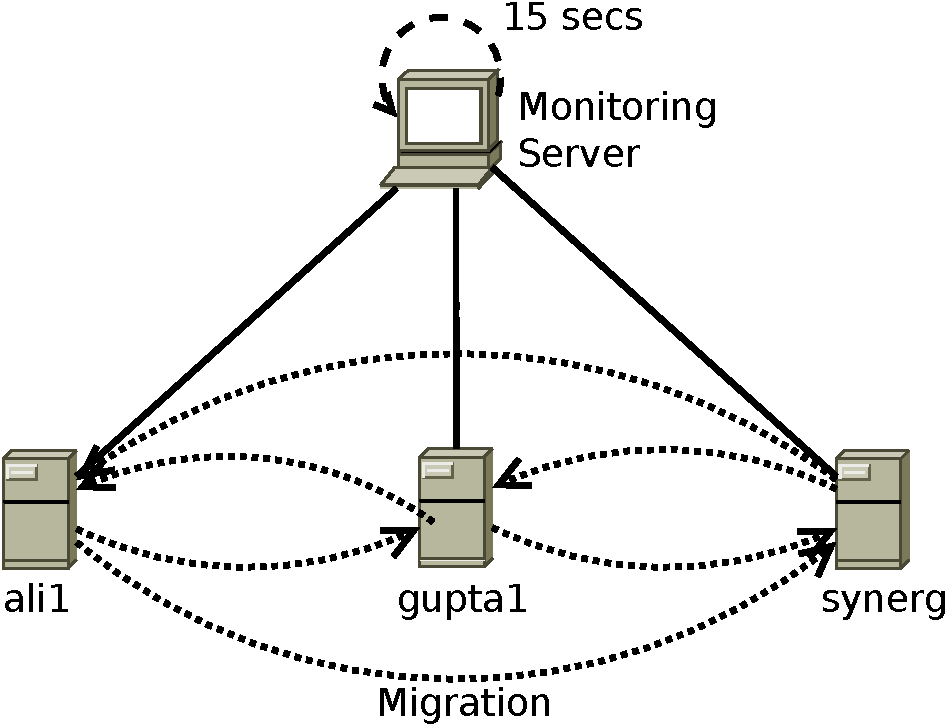
\includegraphics[scale=0.6]{system}
  \caption{System Overview}
\end{figure}

\section{Implementation Details}
We have used four host machine all with ubuntu 16.04 as OS. For container management (creation, removing, configuration etc.) we have used LXD libraries with pylxd \cite{pylxd} package for the python.

Basic goal of this project was to manage the resource of across the different containers by effectively utilizing the resources of the host.
Here is the overview of implementation with their job.

\begin{enumerate}
 \item Their will be one monitoring server which will periodically collect the status of each container of each server for a fixed interval of time. Status will include average CPU and memory usage of that container over the specific period of time.
 
 \item Then monitoring server will analyze the statistics for finding out which containers are overload and which are underloaded.
 
 \item Our key focus is to meet the SLA requirement of maximum overloaded containers at given time rather than meeting only few highly overloaded containers. So, overload containers list is sorted ascending order of their usage(like memory usage).
 
 \item For each server's overloaded containers 3 step optimization process is used.
 \begin{enumerate}
  \item \textit{OneToOne Resizing}: For every overloaded container we find one underload container (within same host) from whom we take the resources and assign to it. If no underload load container is found then it is added into "Remaining Queue"(RQ).
  
  \item \textit{ManyToOne Resizing}: For every overloaded container in RQ which are added by step (a), we try find multiple underload containers (within same host) whose combined resources can be  assign to it. If no underload load container is found then it is added into "Remaining Queue" (RQ).
  
  \item \textit{Migration and Resizing}: For every overloaded container in RQ which are added by step (b), we try find the first underload server where the container can be migrated. Then we live migrate that container to the new location. After the migration we do Resizing using step (a) and (b).
 \end{enumerate}
\end{enumerate}

\noindent Method for finding underloaded and overloaded containers:

\noindent We have three constants:
\begin{enumerate}
 \item Threshold percentage $(t)$: If utilization is greater than $t$ then we will call that container is overloaded with some exceptional condition discussed in SLA.
 \item Underload Gap percentage $(u)$: For underloaded containers, minimum gap percent between utilization and threshold i.e  $threshold - utilization < u$ (unit is percent)
 \item Overload Gap Percentage $(o)$: For overload container, minimum gap percent between utilization and thershold i.e  $utilization -threshold > o$ (unit is percent)
\end{enumerate}
\noindent SLA specification $(sla)$ is provided by the user.

\noindent Its a requirment given by client at the time of creation of the containers. Example, Memory SLA saying 1024MB means that container should be allocated 1024MB. If that container has $utilization > t$ then it will not be considered as an overloaded container as size of container is as per the SLA.

\begin{figure}[!htb]
  \centering
  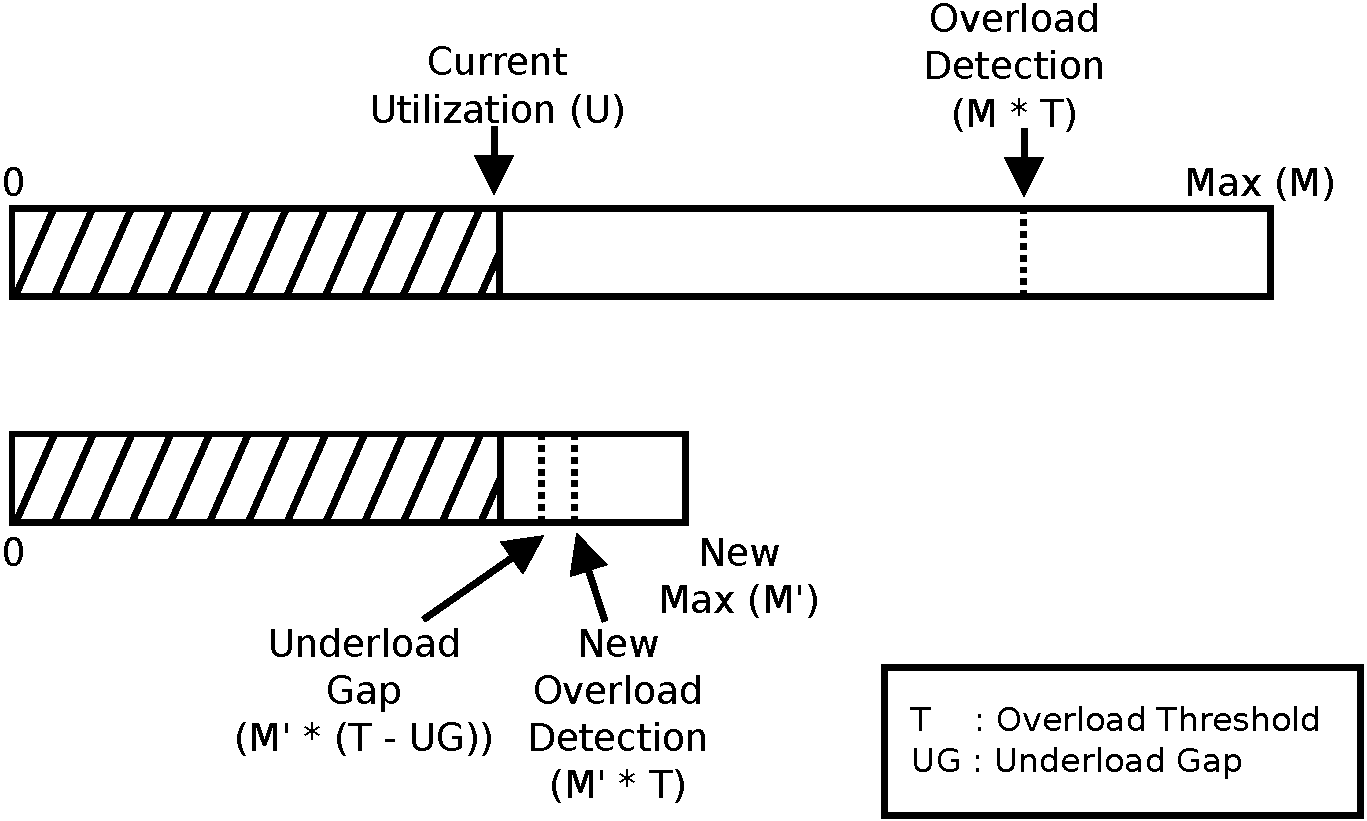
\includegraphics[scale=0.5]{underload}
  \caption{Potential underloaded resource pre-emption}
  \label{fig:underload}
\end{figure}

\begin{figure}[!htb]
  \centering
  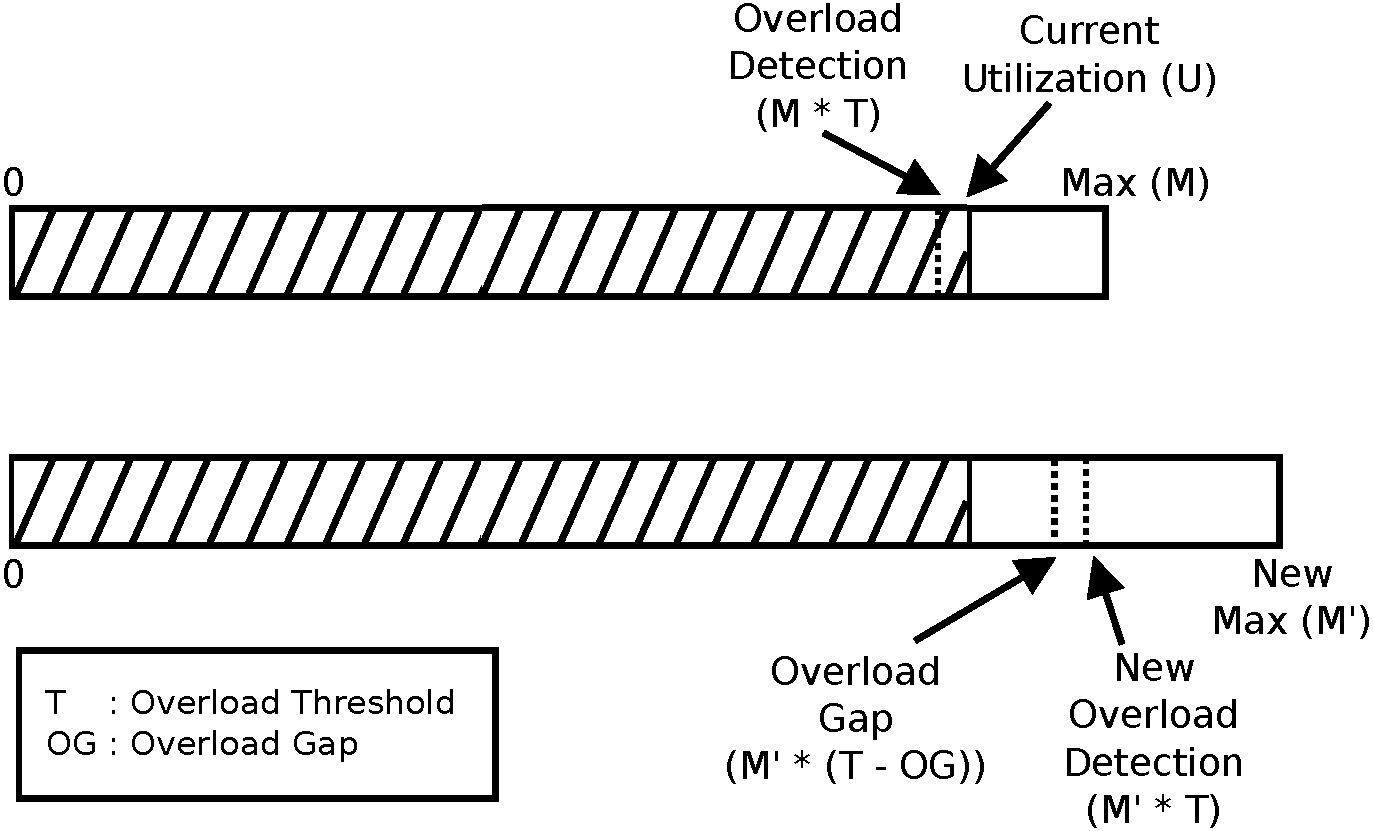
\includegraphics[scale=0.5]{overload}
  \caption{Potential overloaded resource allocation}
  \label{fig:overload}
\end{figure}

\section{Experimentation and Inferences}
Since our implementation only considers vertical resolution of hotspots, our experimental setup has 4 containers running on one machine each having SLA of 2 CPUs and 1024MB memory. Considering the overcommitment of memory, current allocated memory to 2 containers (say $c1$ and $c2$) are 512MB and remaining 2 containers (say $c3$ and $c4$) have complete 1024MB.

We generate synthetic load using \textit{stress} \cite{stress} utility. Load value is randomly generated and each load lasts for 20 seconds. We gather the statistics of which containers are underloaded, which are overloaded, their utilization, current allocated memory and how much memory is being utilized.

Parameters varied are Underload Gap (UG) and Overload Gap (OG) to see how many times the containers go in overload state and whether the hotspot from overloaded containers can be alleviated or not.

Since $c3$ and $c4$ are alloted the maximum memory at the beginning, they will not be considered as overloaded. But as $c1$ and $c2$ are not being alloted their maximum value, they may show up as overload. As iterations proceed potentially all containers can be overloaded.

First we varied UG from 5\%, 10\%, 15\% and 20\%. 

\begin{table}[!htb]
  \centering
  \begin{tabular}{cc}
  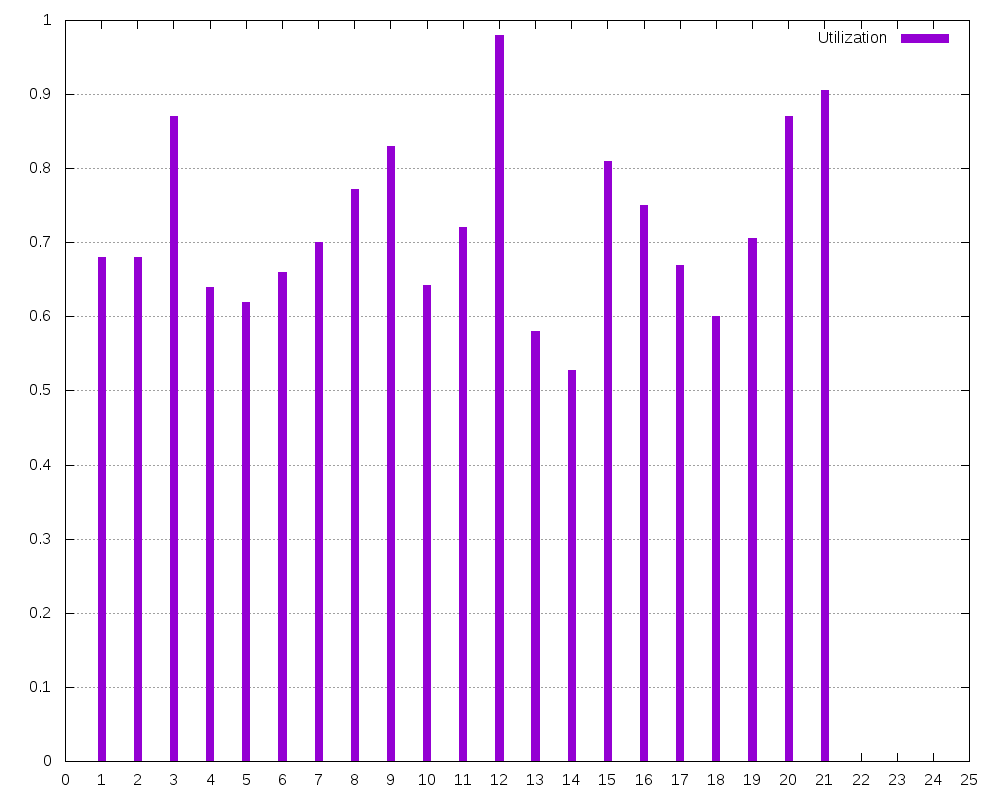
\includegraphics[scale=0.2]{cp1479681211168_5} & 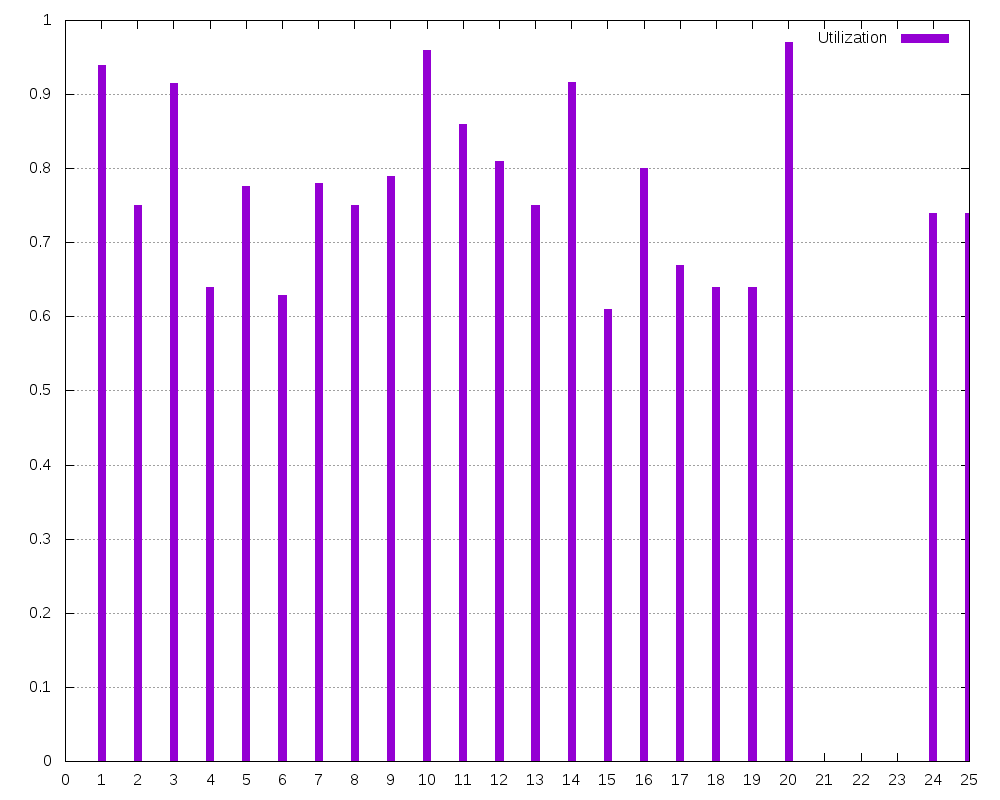
\includegraphics[scale=0.2]{cp1479681211168_10} \\
  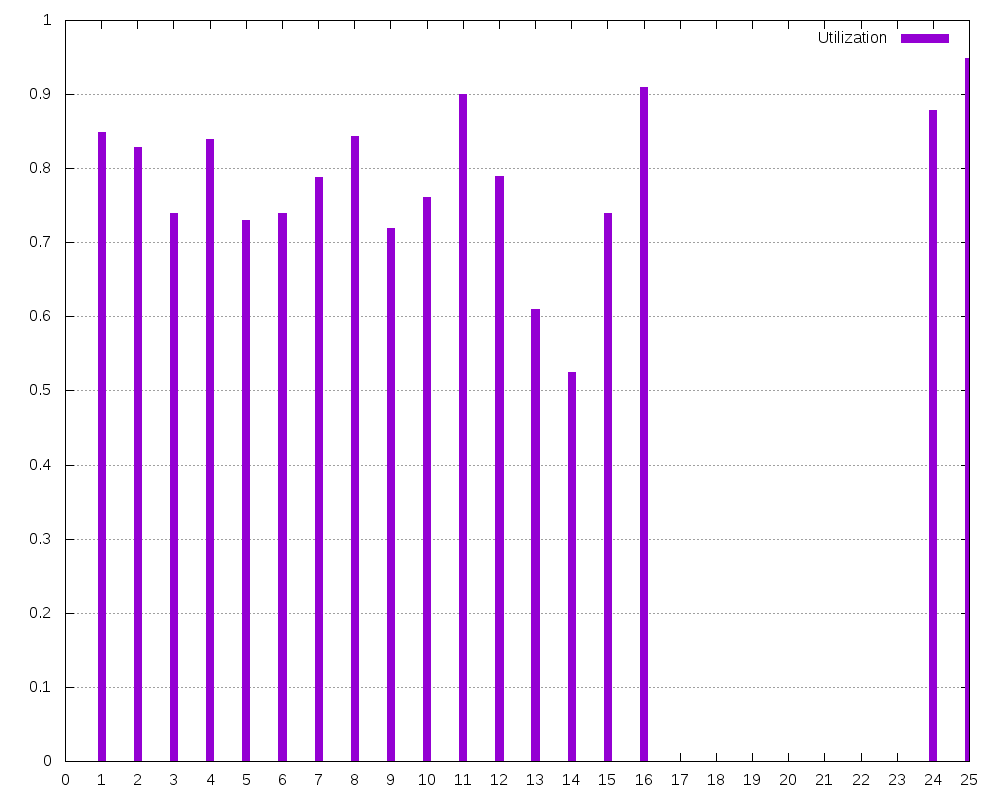
\includegraphics[scale=0.2]{cp1479681211168_15} & 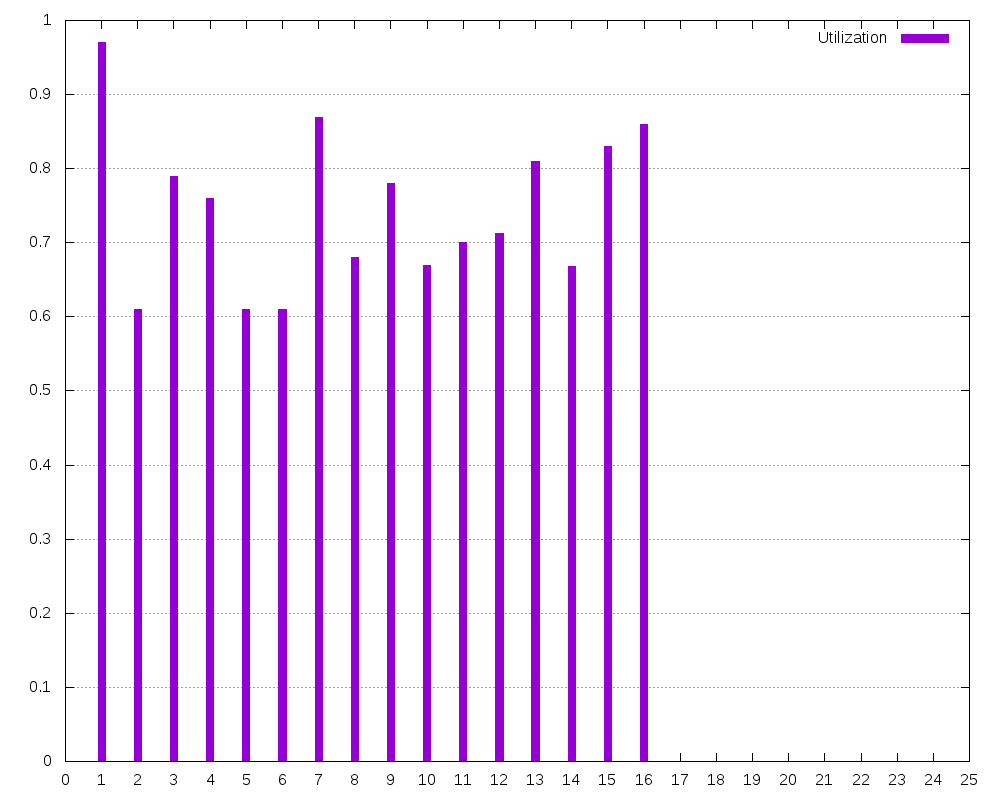
\includegraphics[scale=0.2]{cp1479681211168_20} \\
  \end{tabular}
  \caption{Increase in number of overloads of a container - 5\%, 10\%, 15\% and 20\%}
\end{table}

\newpage
\bibliographystyle{unsrt}
\bibliography{References}
\newpage

\end{document}